\documentclass[../ZF_SWEN1.tex]{subfiles}

\begin{document}
\begin{figure}[H]
\centering
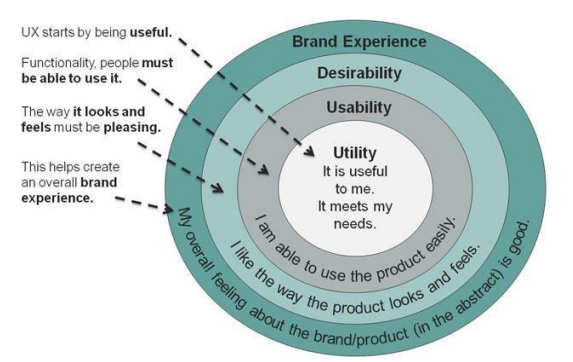
\includegraphics[width=0.3\textwidth]{Resources/Images/Usability.png}
\caption{\label{fig:Usability}Usability.}
\end{figure}


\subsection{Usability}
\textbf{Definition: } Effektivität, Effizienz, Zufriedenheit -> Ziele erreichen im spezifischen Kontext \\

\begin{itemize}
	\item \textbf{4 wichtige Aspekte}
	\begin{itemize}
		\item Benutzer
		\item Seine Ziele/Aufgaben
		\item Sein Kontext
		\item Softwaresystem (inkl.UI)
	\end{itemize}
\end{itemize}


\subsection{Usability Engineering}

\textbf{Ziel: } Software entwickeln, die drei Anfroderungen erfüllt

\begin{itemize}
	\item \textbf{Drei Anforderungen: }
	\begin{itemize}
		\item Effektivität
		\begin{itemize}
			\item Aufgaben vollständig erfüllen
			\item Genauigkeit
		\end{itemize}
	
		\item Effizienz
		\begin{itemize}
			\item Mit minimalem Aufwand (Mental, Physisch, Zeit)
		\end{itemize}
					\item Zufriedenheit 
		\begin{itemize}
			\item \textbf{Minimum: } nicht verärgert
			\item \textbf{Normal: } Zufrieden
			\item \textbf{Optimal: } Erfreut
		\end{itemize}

	\end{itemize}

\end{itemize}


\subsection{Usability Anforderungen}

\begin{itemize}
	\item \textbf{7 Anforderungen:}
	\begin{itemize}
		\item Aufgabengemessenheit
		\item Lernförderlichkeit
		\item Individualisierbarkeit
		\item Erwartungskonformität
		\item Selbstbeschreibungsfähigkeit
		\item Steuerbarkeit
		\item Fehlertoleranz
	\end{itemize}
\end{itemize}


\subsubsection{Aufgabenangemessenheit}
\begin{itemize}
	\item Minimale Anz. Schritte f. Aufgabe
	\item Nur wichtige Informationen
	\item Kontextabhängige Hilfe
	\item Minimale Anz. Benutzereingaben
	\begin{itemize}
		\item Jede Eingabe nur 1x
		\item Standardwerte
		\item Liste vordefinierter Werte (z.B Länder)
		\item Ableitbare Eingaben vorschlagen
	\end{itemize}
\end{itemize}

\subsubsection{Selbstbeschreibungsfähigkeit}
\begin{itemize}
	\item Benutzer ausreichend informieren

	\begin{itemize}
		\item Wo er ist
		\item Was er tun soll / kann
		\item Wie er es tun soll (Formate, Werte)
	\end{itemize}
	
	\item Begriffe des Benutzers verwenden (Labels, Fehlermeldungen)
	\item Affordanzen

\end{itemize}


\subsubsection{Kontrolle}

\begin{itemize}
	\item Mit Interaktion Benutzer steuern
	\begin{itemize}
		\item Initiative, Tempo
		\item Dialogfluss
		\item Darstellungsformate
		\item Inputmodalität (Maus, Tastatur, Touch, Sprache)
	\end{itemize}
	
	\item Benutzeraktionen rückgängig machen können
	\item Benutzeraktionen jeder Zeit abbrechen können
\end{itemize}

\subsubsection{Erwartungskonformität}
\begin{itemize}
	\item Bezüglich
	\begin{itemize}
		\item Design
		\item Interaktion
		\item Struktur
		\item Komplexität
		\item Funktionalität
	\end{itemize}
	\item Konsistenz
	\begin{itemize}
		\item Terminologie
		\item Verhalten (Reihenfolge Aktionen, Änderungen)
		\item Informationsdarstellung (Platzierung, Wortwahl)
	\end{itemize}
\end{itemize}

\subsubsection{Fehlertoleranz}
\begin{itemize}
	\item Benutzerfehler vermeiden
	\begin{itemize}
		\item Klar kommunizieren (Erwarteter Input, Funktionen aktiv resp. sinnvoll)
	\end{itemize}
	\item Benutzereingaben vor Aktion überprüfen
	\item Nicht unbedingt beim Tippen
	\item Benutzer helfen
	\begin{itemize}
		\item Fehler zu erkennen
		\item Ursache zu verstehen
		\item Aus Fehlerzustand zu kommen
	\end{itemize}
	\item Einfache Korrektur
	\item Kein Datenverlust
\end{itemize}

\subsubsection{Individualisierbarkeit}
\begin{itemize}
	\item System anpassbar sein:
	\begin{itemize}
		\item Know-How
		\item Sprache
		\item Kultur
		\item Benutzer mit Einschränkungen
	\end{itemize}	
\end{itemize}

\subsubsection{Lernförderlichkeit}
\begin{itemize}
	\item Informationen über unterliegende Konzepte und Regeln anbieten
	\begin{itemize}
		\item Um mentales Modell anzugleichen
		\item Nur auf Verlangen des Users
		\item eifache Tasks ohne Vorkentnisse
		\item komplexere Konzepte bei der Verwendung zu erlernen
	\end{itemize}
\end{itemize}





















































\end{document}